\section{Screen Captures}

	\normalsize
	{
		In Fig. \ref{fig:SSLoadingScreen} we can see the application loading.  
		The splash screen shows the dynamic link libraries being loaded.  During this process
		types are inspected via reflection for architectural interfaces.
		\newline			
	}

	\begin{figure}[h!]
		\centering
		
\includegraphics[scale=0.9]{pages/appendix3/figures/lgpscreens/loading.png}
		\caption{Loading screen}
		\label{fig:SSLoadingScreen}
	\end{figure}
		
	\normalsize
	{
		In Fig. \ref{fig:SSWindow} the interface can be seen.  At this stage the panels
		are not visible however are present and waiting for menu events to load the appropriate panes
		and place the UserControl into the panes tab control.
		\newline			
	}
		
	\begin{figure}[h!]
		\centering
		
\includegraphics[scale=0.70]{pages/appendix3/figures/lgpscreens/main.png}
		\caption{Main window}
		\label{fig:SSWindow}
	\end{figure}
	
	\newpage

	\normalsize
	{
		Here in Fig. \ref{fig:SSLanguageAndServer}, the main preferences, the user is able to select the preferred language 
		and choose a server to connect to.
		\newline			
	}
				
	\begin{figure}[h!]
		\centering
		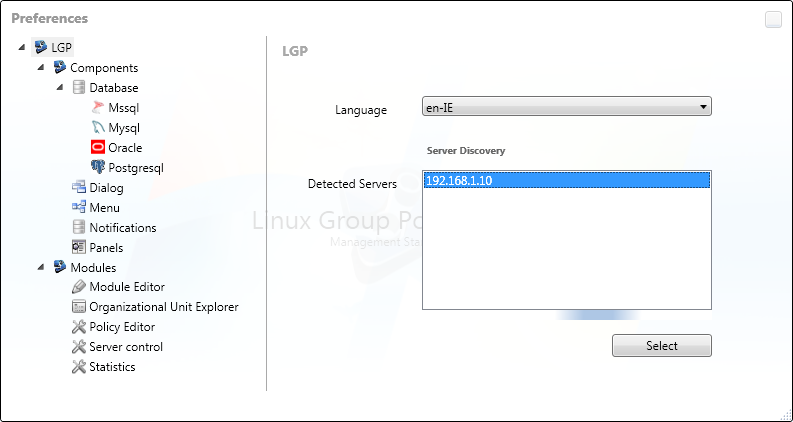
\includegraphics[scale=0.75]{pages/appendix3/figures/lgpscreens/prefs-main.png}
		\caption{Preferences Main}
		\label{fig:SSLanguageAndServer}
	\end{figure}
		
	\normalsize
	{
		In Fig. \ref{fig:SSDb}, the detected database strategy contexts have been detected and selection of the 
		preferred database type is chosen along with the typical database settings.  On the left we can also see the modules themselves
		which may provide context specific configuration elements.
		\newline			
	}		

	\begin{figure}[h!]
		\centering
		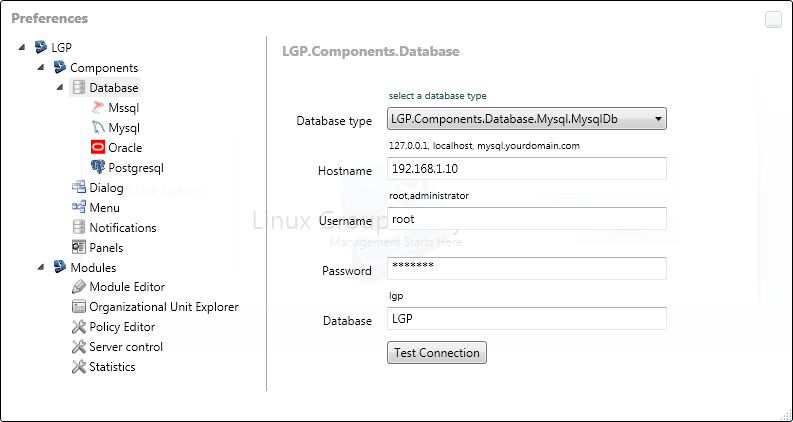
\includegraphics[scale=0.75]{pages/appendix3/figures/lgpscreens/prefs-db.png}
		\caption{Preferences Database}
		\label{fig:SSDb}
	\end{figure}
	
	\newpage
		
	\normalsize
	{
		In Fig. \ref{fig:SSModuleEditor} / \ref{fig:SSModuleEditor2}, the module editor is visible, on the right hand side we have the list of modules on the server.
		On the right hand side is the detected grammar in the module, and available in the middle is the editing area.
		\newline			
	}		

	\begin{figure}[h!]
		\centering
		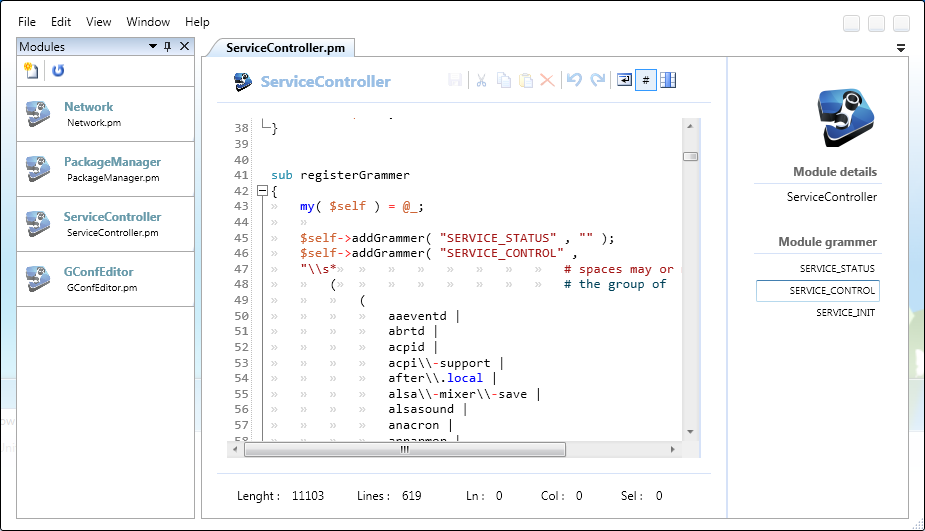
\includegraphics[scale=0.65]{pages/appendix3/figures/lgpscreens/moduleed-edit.png}
		\caption{Module editor}
		\label{fig:SSModuleEditor}
	\end{figure}
	
	\begin{figure}[h!]
		\centering
		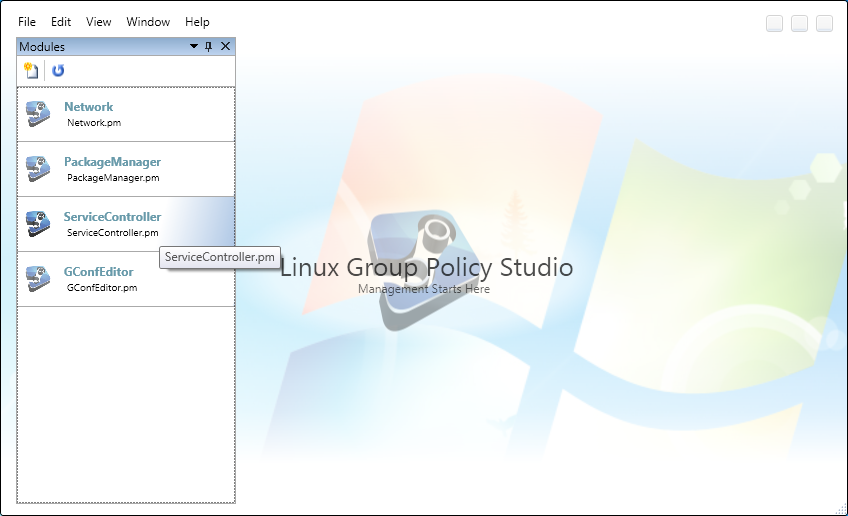
\includegraphics[scale=0.70]{pages/appendix3/figures/lgpscreens/moduleed-list.png}
		\caption{Module list}
		\label{fig:SSModuleEditor2}
	\end{figure}
	
	\newpage
		
	\normalsize
	{
		In Fig. \ref{fig:SSouDragDRop} / \ref{fig:SSClient} , the admin is showing off the drag and drop adorner.  
		A client machine is being drag into another ou, also the client information on the side has been activated.
		The unique machine identifier along with the distribution and Perl client info is available.
		\newline			
	}		

	\begin{figure}[h!]
		\centering
		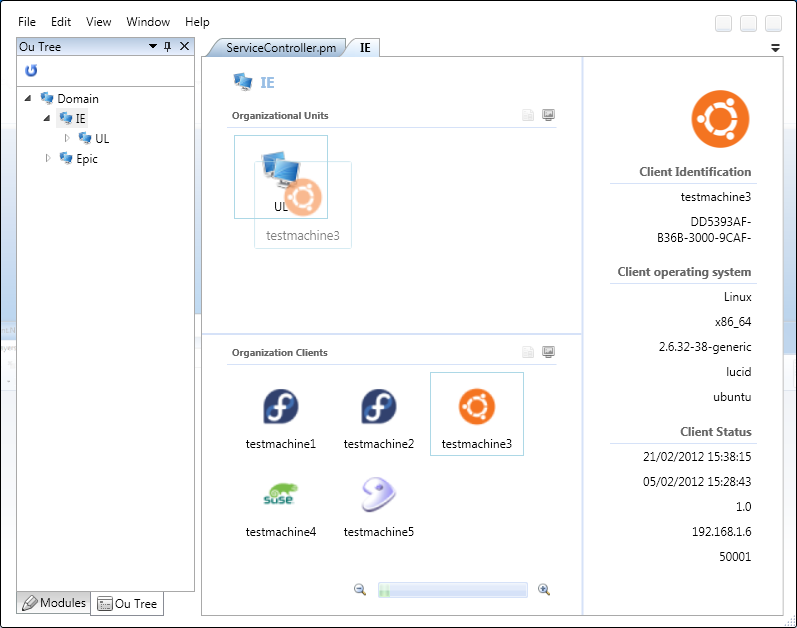
\includegraphics[scale=0.60]{pages/appendix3/figures/lgpscreens/ou-dragdrop-adorner.png}
		\caption{Ou - Drag / drop}
		\label{fig:SSouDragDRop}
	\end{figure}
	
	\begin{figure}[h!]
		\centering
		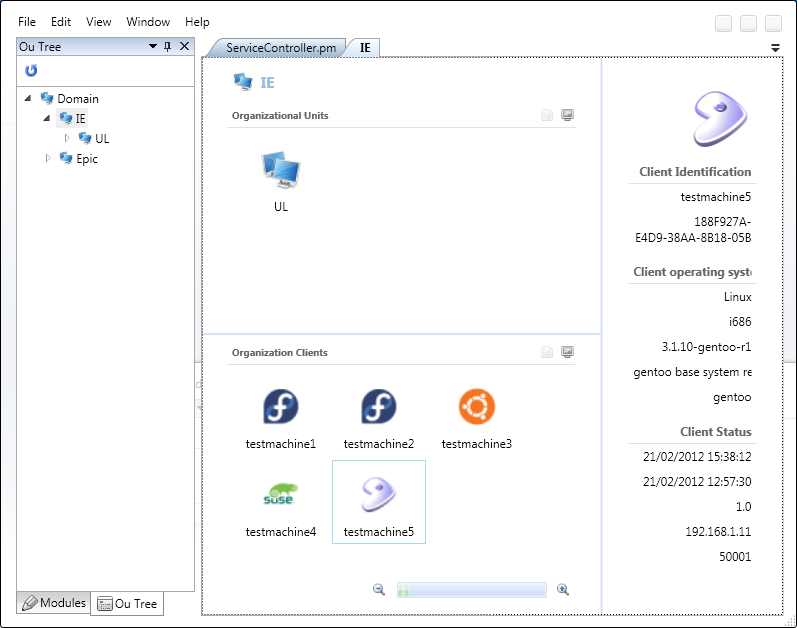
\includegraphics[scale=0.60]{pages/appendix3/figures/lgpscreens/ou-explorer-client.png}
		\caption{Ou - Client}
		\label{fig:SSClient}
	\end{figure}
	
	\newpage
		
	\normalsize
	{
		In Fig.\ref{fig:SSOuMenuOptions}, The limited organizational unit information is available.
		In later revisions it will show clients and sub OUs etc. The organizational menu options are visible.
		The options provided by the Organizational Unit Explorer Plug-in are seen as well as 
		menu options provided by the policy editor
		\newline			
	}
	
	\begin{figure}[h!]
		\centering
		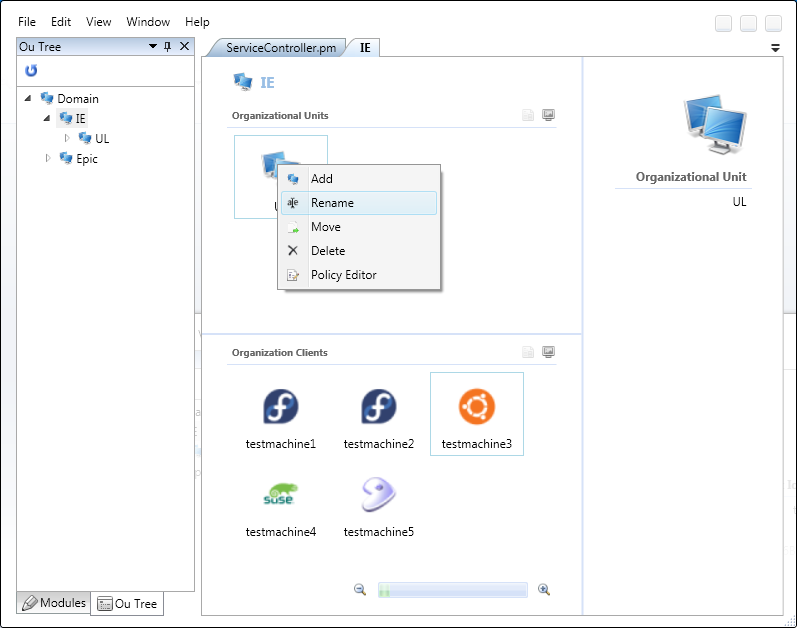
\includegraphics[scale=0.6]{pages/appendix3/figures/lgpscreens/ou-menu-options.png}
		\caption{Ou - options}
		\label{fig:SSOuMenuOptions}
	\end{figure}
	
	\normalsize
	{
		The following three figures \ref{fig:SSOuAdd} / \ref{fig:SSOuDelete} / \ref{fig:SSOuMove} , 
		depict the organizational pop up windows for the adding, moving and deleting of OUs respectively.	
	}
	
	\begin{multicols}{2}
	
		\begin{figurehere}
			\centering
			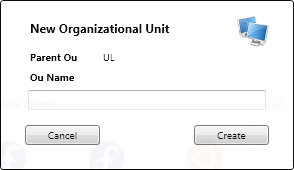
\includegraphics[scale=0.8]{pages/appendix3/figures/lgpscreens/ou-add.png}
			\caption{Ou - add}
			\label{fig:SSOuAdd}
		\end{figurehere}
		
		\vspace{3mm}
		\begin{figurehere}
			\centering
			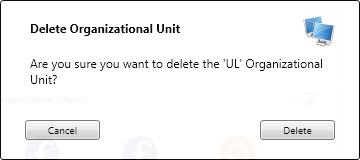
\includegraphics[scale=0.8]{pages/appendix3/figures/lgpscreens/ou-delete.png}
			\caption{Ou - delete}
			\label{fig:SSOuDelete}
		\end{figurehere}
		
		\columnbreak
		
		\begin{figurehere}
			\centering
			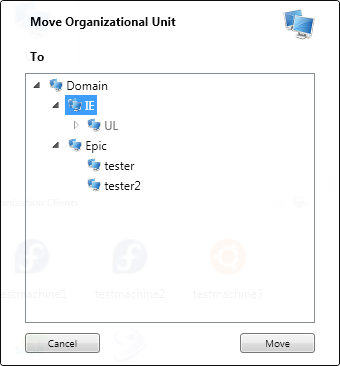
\includegraphics[scale=0.8]{pages/appendix3/figures/lgpscreens/ou-move.png}
			\caption{Ou - move}
			\label{fig:SSOuMove}
		\end{figurehere}
			
	\end{multicols}


	\normalsize
	{
		Here in Fig. \ref{fig:SSPolicyEditor} the administrator has created an invalid rule
		as indicated by the red high light. The rules are visible on the right hand side as well
		as the code editor.
		\newline			
	}

	\begin{figurehere}
		\centering
		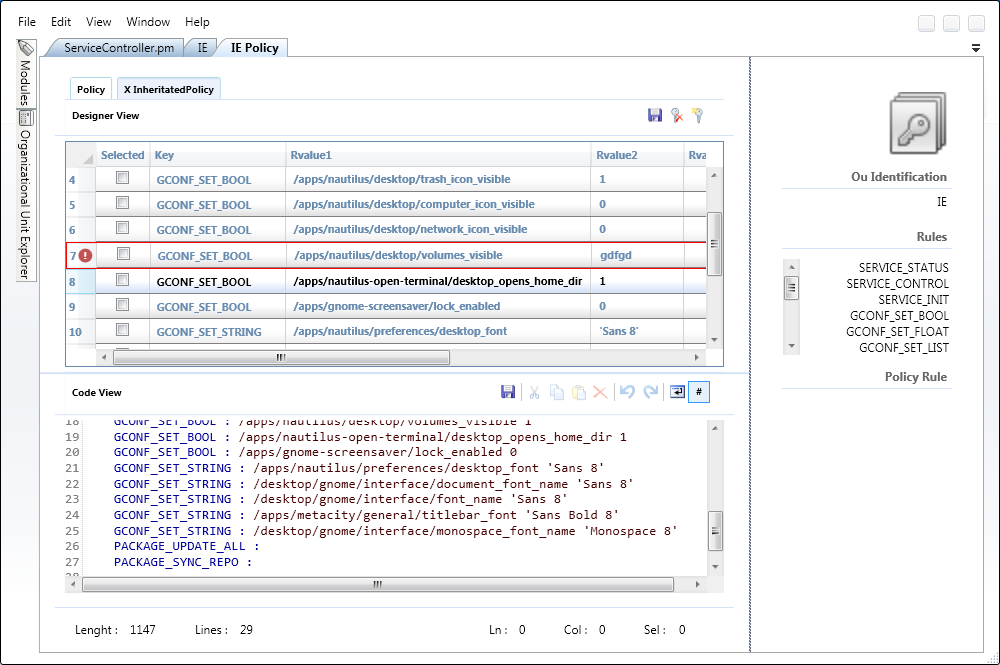
\includegraphics[scale=0.5]{pages/appendix3/figures/lgpscreens/policy-editor.png}
		\caption{Ou - policy editor}
		\label{fig:SSPolicyEditor}
	\end{figurehere}

	
	\normalsize
	{
		Fig. \ref{fig:SSServerControl} depicts the push features provided by the Server Control Module
		Stress testing features are available also.
		\newline			
	}

	\begin{figurehere}
		\centering
		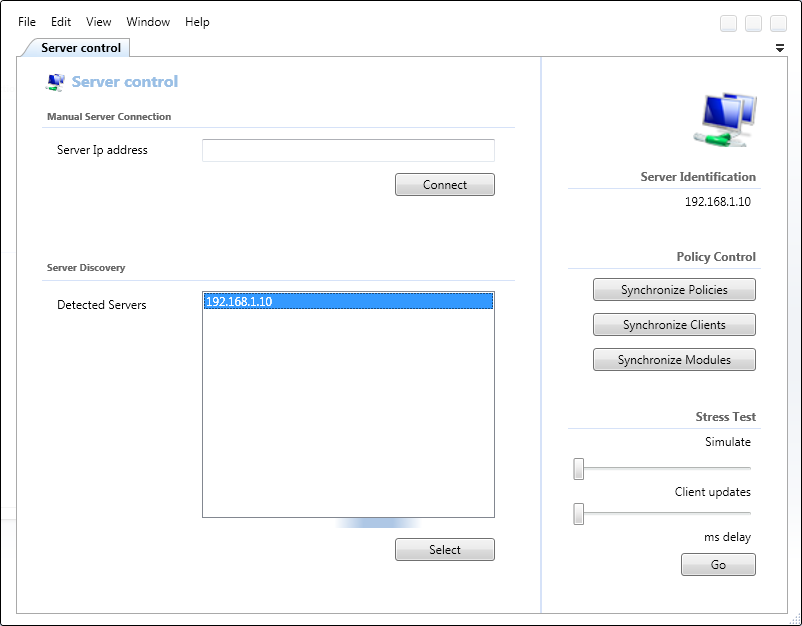
\includegraphics[scale=0.65]{pages/appendix3/figures/lgpscreens/servercontrol.png}
		\caption{Ou - Server Control}
		\label{fig:SSServerControl}
	\end{figurehere}
	
	\normalsize
	{
		Fig. \ref{fig:SSStatistics} shows the monitoring of the server, three simple statistics
		are provided, the queue size on the server, network usage and the processor usage.
		\newline			
	}

	\begin{figurehere}
		\centering
		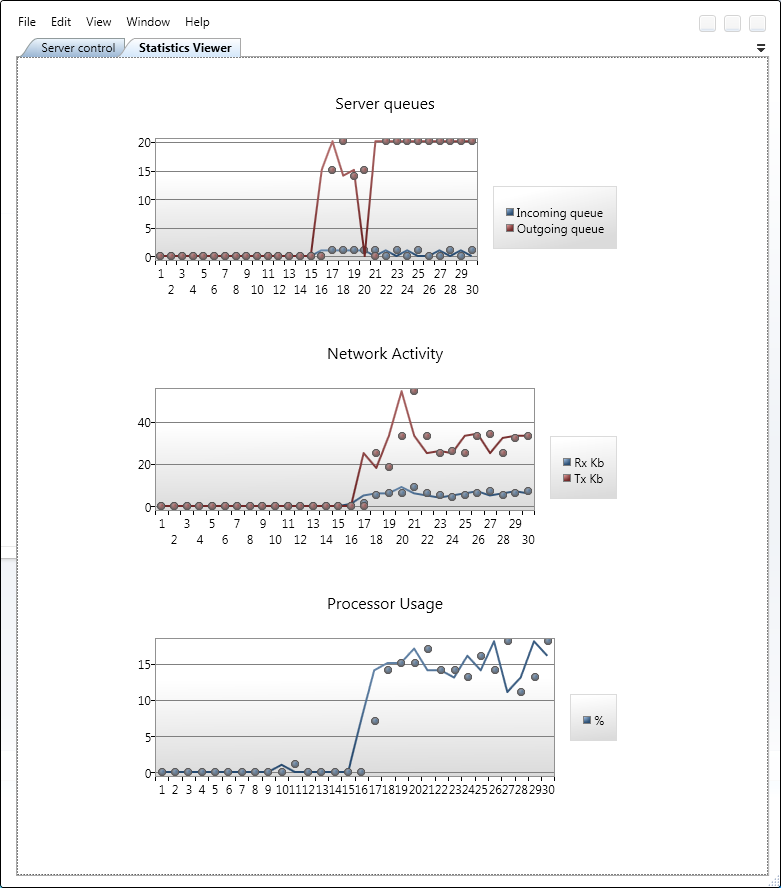
\includegraphics[scale=0.75]{pages/appendix3/figures/lgpscreens/statistics.png}
		\caption{Ou - Statistics}
		\label{fig:SSStatistics}
	\end{figurehere}

\newpage